\documentclass[a4paper]{article}
\usepackage{graphicx}
\usepackage{onecolpceurws}
\usepackage{url}
\usepackage{hyperref}

\title{The TTC 2014 Movie Database Case}

\author{
Tassilo Horn\\ University of Koblenz-Landau\\ Germany\\ horn@uni-koblenz.de
\and
Christian Krause\\ SAP Innovation Center\\ Germany\\ christian.krause01@sap.com
\and
Matthias Tichy\\ Chalmers / University of Gothenburg\\ Sweden\\ matthias.tichy@cse.gu.se
}

\institution{}

\begin{document}
\maketitle

\begin{abstract}
This is the movies case for the TTC 2014.
\end{abstract}
\vskip 32pt


\section{Introduction}


\section{Detailed Case Description}

The transformation is on data from a movie database.
We use the metamodel shown in Figure~\ref{fig:metamodel}.
We generate synthetic test data and also use real data
from the IMDB movie database. You can use the EMF model and
parser provided in \cite{IMDB2EMF} for this purpose.


\begin{figure}[ht]
\centering
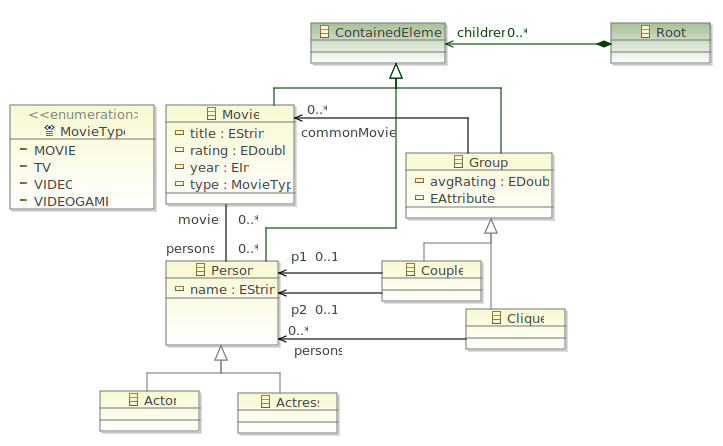
\includegraphics[width=0.6\textwidth]{movies}
\caption{Simplified metamodel for the movie database.}
\label{fig:metamodel}
\end{figure}

\subsection{Task 1: Generating Test Data}
\label{sec:gen-test-data}

The first task is to generate some test data.
This will be used to test the correctness and to do benchmarks later.
The generation of the test data should go as follows...
A graphical Henshin specification is shown in Figure~\ref{fig:gen-test-data}

\begin{figure}[p]
\centering
\includegraphics[width=0.8\textwidth]{gen-test-data}
\caption{Henshin specification for generating synthetic movie test data.}
\label{fig:gen-test-data}
\end{figure}

\subsection{Task 2: Finding Couples}

\subsection{Task 3: Computing Rankings}

\section{Evaluation Criteria}

\subsection{Completeness \& Correctness}

Correctness is checked using the synthetic data.

\subsection{Benchmarks}

Perform benchmarks using the following input data sets:
\begin{enumerate}
\item the synthetic data generated in Section~\ref{sec:gen-test-data}, and 
\item the IMDB data (available at \cite{IMDBDATA}; parse, e.g., using \cite{IMDB2EMF}).
\end{enumerate}
For both cases, you should run the transformation and measure 
the time needed to complete the transformation (without loading 
and saving the model).

There are two versions of the transformations: Task 1 and Task 1+2.
Please run the benchmarks for both versions and both data sets.

Plot the benchmarks. On the x-axis you print the size of the data set
in number of nodes and on the y-axis you plot the time. The number of nodes
includes all types of nodes (movies and actors). Make the measurements in
steps of 100,000 nodes. For the synthetic data, choose n=?,...,?
For the IMDB data, take the whole data set and to sampling. You can use
the sampler provided in \cite{IMDB2EMF}. 

NOTE TO US: IMPLEMENT SAMPLING!



\bibliographystyle{plain}
\bibliography{biblio}

\end{document}


